\begin{figure}
    \centering
    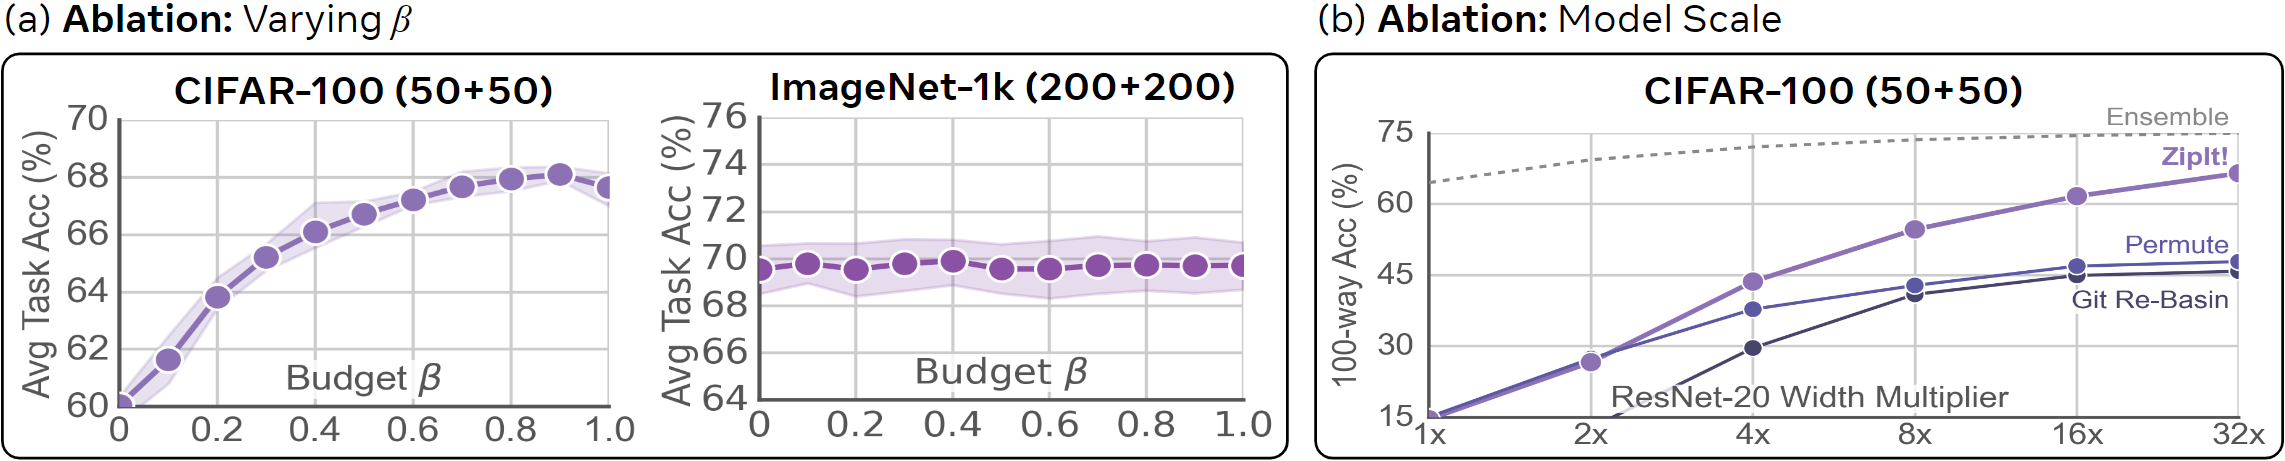
\includegraphics[width=\linewidth]{figures/imgs/varying_beta_and_scale.png}
    \caption{{\bf Varying $\beta$ and Model Scale.} 
    Left: 
    % we test the importance of same model matches by varying the budget $\beta$. A budget of 0 means no same-model matches are allowed, while 1 places no restrictions. 
    We find when the model has enough capacity for the task, a high budget (Sec.~\ref{sec:partial_zip}) improves performance. 
    Right: 
    \name{}\ makes effective use of extra model capacity to quickly reach the ensemble on CIFAR-100 (50+50) when we increase the width of ResNet-20 models. 
    In contrast, our baselines only slightly benefit from the extra scale.
    % Git Re-Basin \cite{ainsworth2022git} and Permute only slightly benefit from the extra scale.
% Git Re-Basin \cite{ainsworth2022git} and Permute only slightly benefit from the extra scale.
    }
    \label{fig:variations}
    % \vspace{-10pt}
\end{figure}

% \begin{figure}
%     \centering
%     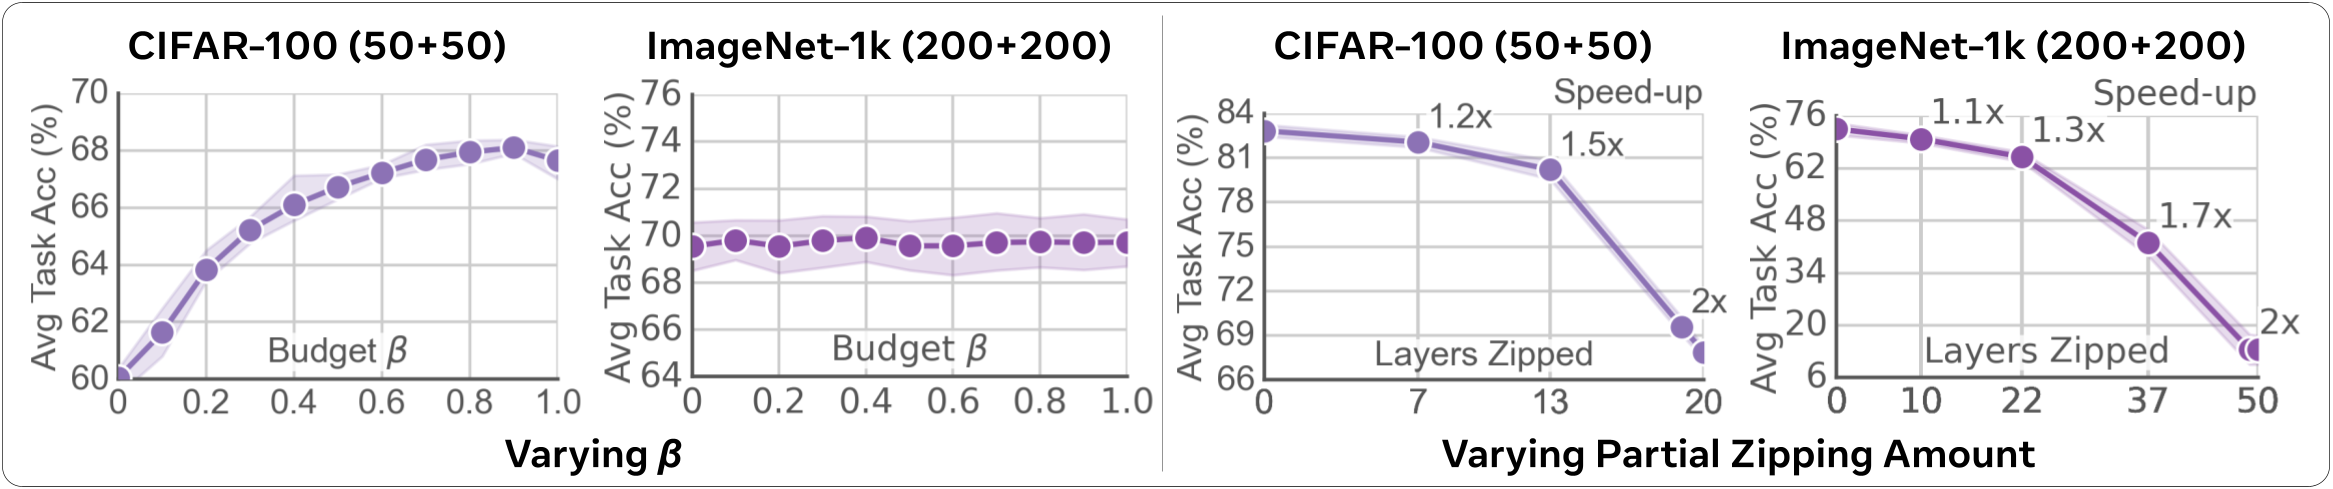
\includegraphics[width=\linewidth]{figures/imgs/zipit_varying_ablations.png}
%     \caption{{\bf Varying $\beta$ and Partial Zipping} (Sec.~\ref{sec:partial_zip}). Left: we test the importance of same model matches by varying the budget $\beta$. A budget of 0 means no same-model matches are allowed, while 1 places no restrictions. We find when the model has enough capacity for the task, a high budget improves performance. Right: by leaving some layers unzipped, we can recover a significant amount of performance while still merging most of the model. 
%     }
%     \label{fig:variations}
% \end{figure}


% \begin{figure}
%     \begin{minipage}[t]{0.48\linewidth}
%         \centering
%         \subfloat[
%             \textbf{CIFAR-100 50+50.}
%             \label{fig:budget_ablation_cifar100}
%         ]{
%             \centering
%             \begin{minipage}{0.48\linewidth}{
%                 \centering
%                 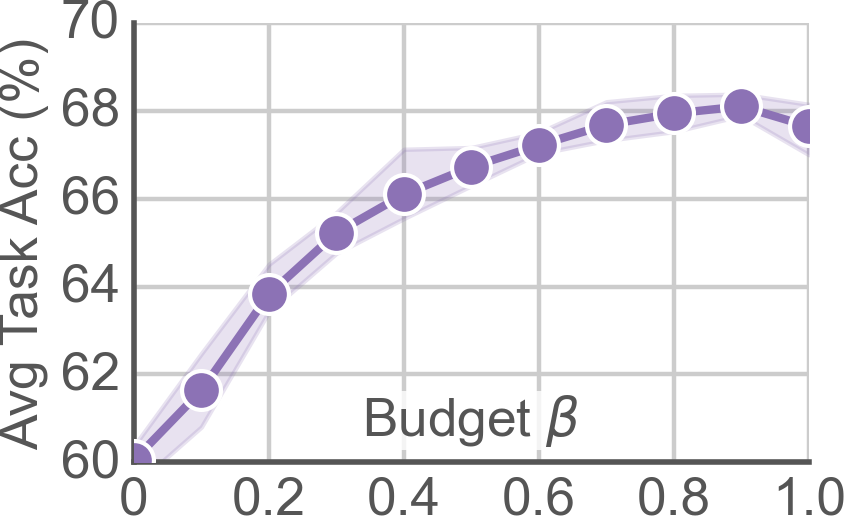
\includegraphics[width=\linewidth]{figures/imgs/cifar100_budget.png}
%             }\end{minipage}
%         }
%         \subfloat[
%             \textbf{ImageNet-1k 200+200.}
%             \label{fig:budget_ablation_imagenet}
%         ]{
%             \centering
%             \begin{minipage}{0.48\linewidth}{
%                 \centering
%                 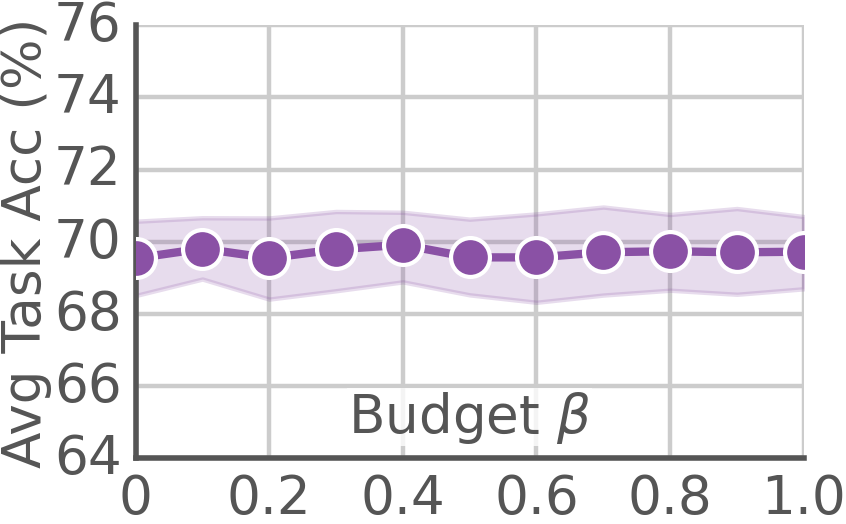
\includegraphics[width=\linewidth]{figures/imgs/imnet_budget.png}
%             }\end{minipage}
%         }
%         \caption{{\bf Varying $\beta$.} We test the importance of same model matches by varying the budget $\beta$ (Sec.~\ref{sec:partial_zip}). A budget of 0 means no same-model matches are allowed, while 1 places no restrictions. We find when the model has enough capacity for the task, a high budget improves performance. }
%         \label{fig:budget_ablation}
%         % \vspace{-80pt}
%     \end{minipage}
%     \hspace{1pt}
%     % \vspace{1em} % Add vertical space between the images
%     \begin{minipage}[t]{0.48\linewidth}
%         \centering
%         \subfloat[
%             \textbf{CIFAR-100 50+50.}
%             \label{fig:partial_zip_cifar100}
%         ]{
%             \centering
%             \begin{minipage}{0.49\linewidth}{
%                 \centering
%                 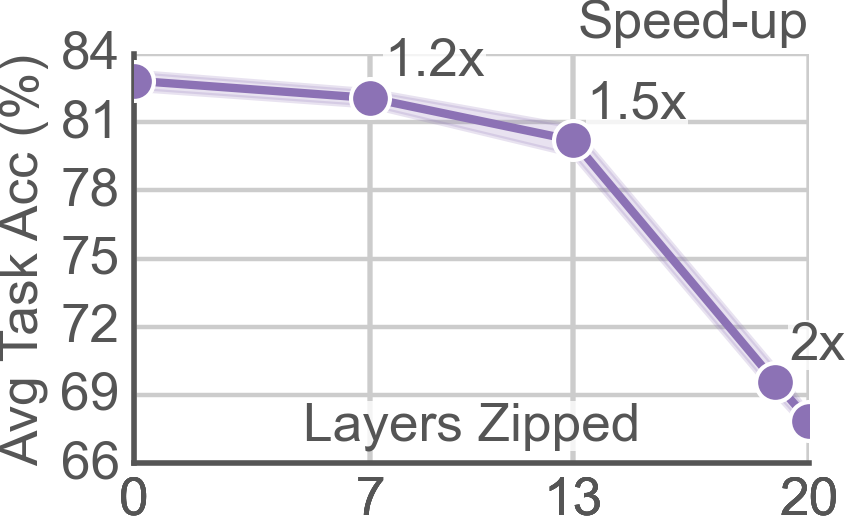
\includegraphics[width=\linewidth]{figures/imgs/partial_zip_CIFAR_50_50.png}
%             }\end{minipage}
%         }
%         \subfloat[
%             \textbf{ImageNet-1k 200+200.}
%             \label{fig:partial_zip_imagenet}
%         ]{
%             \centering
%             \begin{minipage}{0.49\linewidth}{
%                 \centering
%                 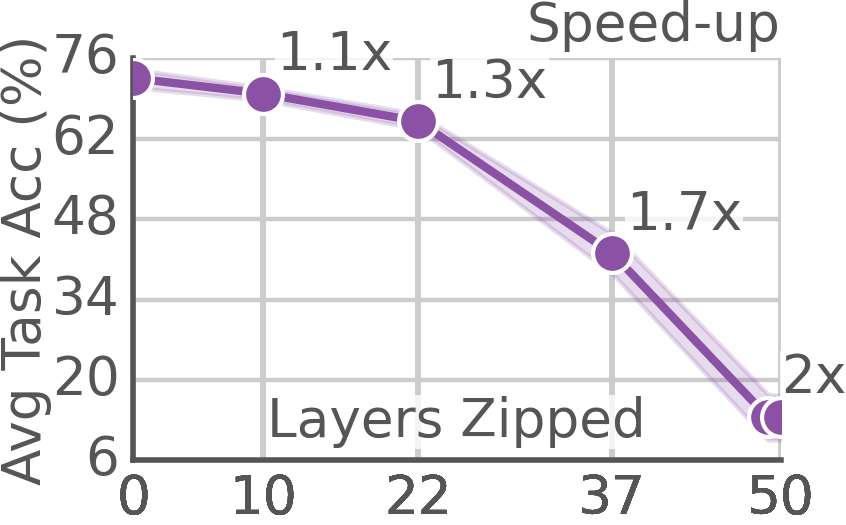
\includegraphics[width=\linewidth]{figures/imgs/partial_zip_imnet_200_200.png}
%             }\end{minipage}
%         }
%         \caption{
%         {\bf Varying Partial Zip.} 
%         By leaving some layers unzipped (Sec.~\ref{sec:partial_zip}), we can recover a significant amount of performance while still merging most of the model. 
%         }
%         \label{fig:varying_partial_zip}
%         % \vspace{10pt}
%     \end{minipage}
%     % \caption{Overall caption for the three images}
%     \vspace{-20pt}
% \end{figure}


%###################



% \begin{figure}[t]
% \centering

% \subfloat[
%     \textbf{CIFAR-100 50+50.}
%     \label{fig:budget_ablation_cifar100}
% ]{
% \centering
% \begin{minipage}{0.48\linewidth}{
% \begin{center}
%     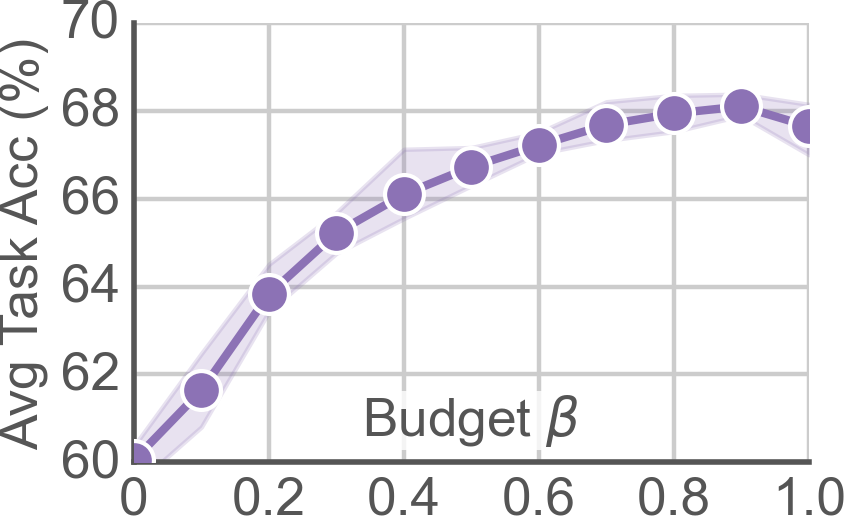
\includegraphics[width=\linewidth]{figures/imgs/cifar100_budget.png}
% \end{center}
% }\end{minipage}
% }
% \subfloat[
%     \textbf{ImageNet-1k 200+200.}
%     \label{fig:budget_ablation_imagenet}
% ]{
% \centering
% \begin{minipage}{0.48\linewidth}{
% \begin{center}
%     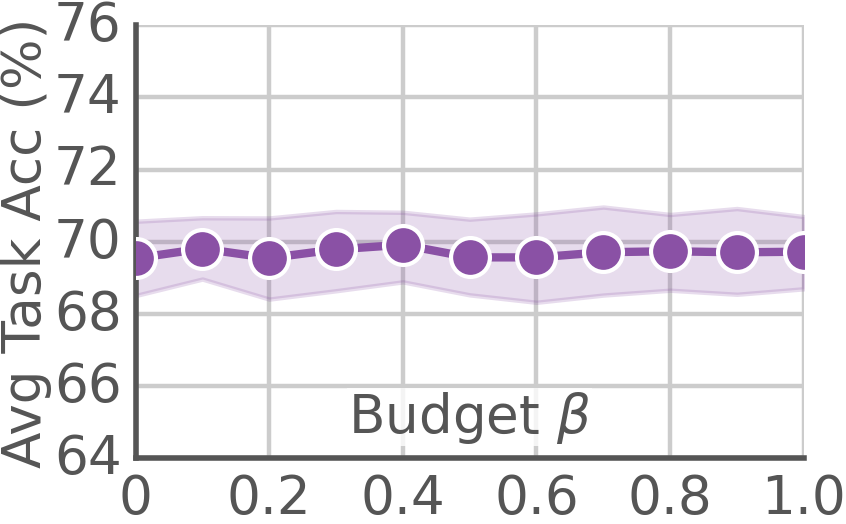
\includegraphics[width=\linewidth]{figures/imgs/imnet_budget.png}
% \end{center}
% }\end{minipage}
% }

% \caption{{\bf Varying $\beta$.} We test the importance of same model matches by varying the budget $\beta$ (Sec.~\ref{sec:partial_zip}). A budget of 0 means no same-model matches are allowed, while 1 places no restrictions. We find when the model has enough capacity for the task, a high budget improves performance. }
% \label{fig:budget_ablation}
% \end{figure}




% \begin{figure}[t]
% \centering

% \subfloat[
%     \textbf{CIFAR-100 50+50.}
%     \label{fig:partial_zip_cifar100}
% ]{
% \centering
% \begin{minipage}{0.49\linewidth}{
% \begin{center}
%     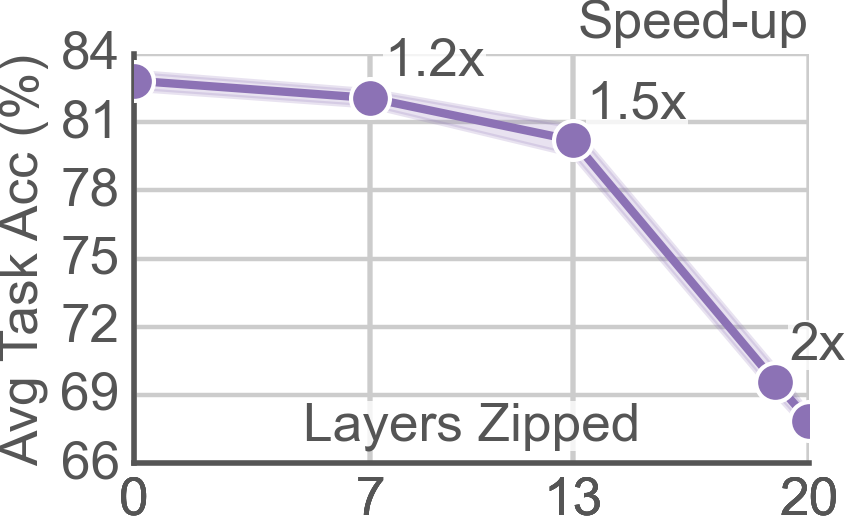
\includegraphics[width=\linewidth]{figures/imgs/partial_zip_CIFAR_50_50.png}
% \end{center}
% }\end{minipage}
% }
% \subfloat[
%     \textbf{ImageNet-1k 200+200.}
%     \label{fig:partial_zip_imagenet}
% ]{
% \centering
% \begin{minipage}{0.49\linewidth}{
% \begin{center}
%     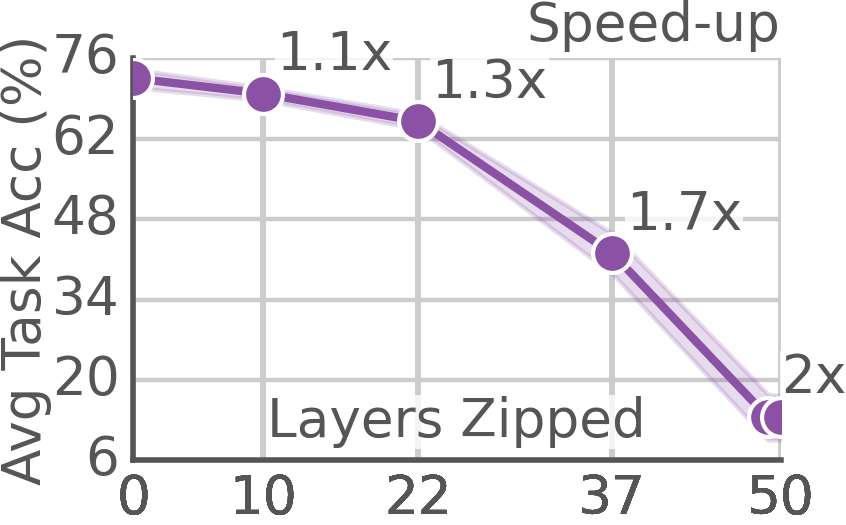
\includegraphics[width=\linewidth]{figures/imgs/partial_zip_imnet_200_200.png}
% \end{center}
% }\end{minipage}
% }

% \caption{
% {\bf Varying Partial Zip.} 
% By leaving some layers unzipped (Sec.~\ref{sec:partial_zip}), we can recover a significant amount of performance while still merging most of the model. 
% }
% \label{fig:varying_partial_zip}
% \end{figure}




% \begin{figure}[t]
% \centering
% %
% \begin{center}
%     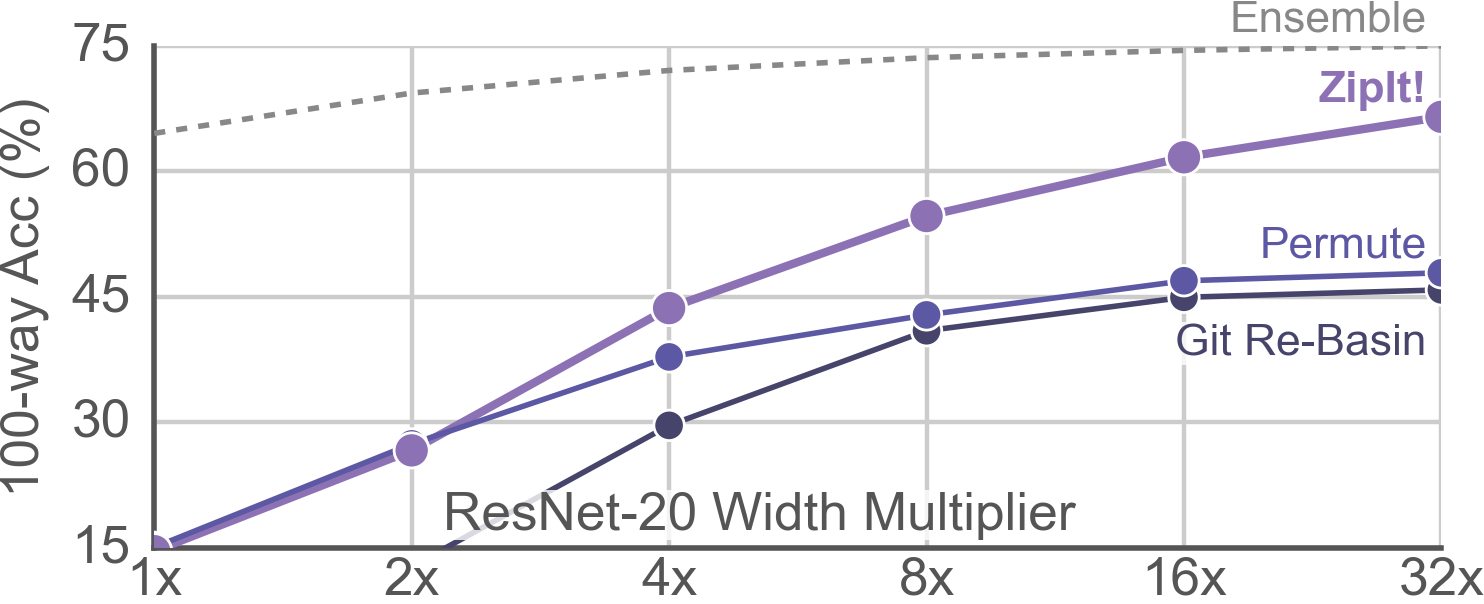
\includegraphics[width=0.95\linewidth]{figures/imgs/model_scale.png}
% \end{center}
% \caption{{\bf Model Scale.} As we increase the width of the ResNet-20 models used for the CIFAR-100 (50+50) setting, \name{}\ makes effective use of that extra capacity, quickly approaching ensemble accuracy. 
% Git Re-Basin \cite{ainsworth2022git} and Permute only slightly benefit from the extra scale.
% }
% \label{fig:model_size}
% \end{figure}

